
\section{OpenETCS process}
\subsection{Motivation}

This document describes the process to  be applied  during the OpenETCS project to achieve the following goals of the OpenETCS project :

\paragraph{A formal reference specification for the ETCS requirements and architecture}
The first goal of the project is to propose a formalization of a subset of the on-board subsystem,
as defined in the SUBSET-26. 

The purpose of the formalization is:
\begin{itemize}
\item to enhance the understanding of modelled subset;
\item to allow formal analysis of the modelled subset;
\item to be able to animate the model for testing an analyzing purpose;
\item to provide information on the completeness and soundness of the SUBSET-26;
\item to be used as a reference formal specification for the implementation of an OBU 
(by the OpenETCS project team and by industrial actors);
\item \dots
\end{itemize}


The output of this goal is a formal specification, understandable by many tools (SCADE, 
Simulink, B tools, OpenETCS tool chain…) that can be given to all railway actors, and 
if possible associated to SRS documents in the ERA database.
The final goal is that industrial actors work with this formal specification instead of 
natural language specification.


\paragraph{Definition of a tool chain and process/methodologies for developing 
on onboard software that can fulfill the EN 50128 requirements}


The process and the associated tools, shall provide a certifiable product. For this purpose all the step of the process and the choice of methods and tools shall be justifyed to ensure a safe approach to build a system.

The full safety process needed for the OpenETCS to be \emph{certifiable} according to CENELEC 50126
and 50128 shall be described in details. This safety plan will detail precisely which activities 
are required or not, why, and the choices that are made that allows to claim that safety is guaranteed.


\paragraph{Building an implementation of the subset of an onboard ETCS using the system model and the 
tool chain}

It is the demonstration that all the work done in the OpenETCS project is coherent, and that
the tool chain is operational.

The output is the result of an implementation for the ETCS requirements and architecture which can be used by the industrial as references.

\paragraph{Define the safety properties at the model level}
In order to comply the CENELEC standards, it is necessary to conduct safety activities 
to identify errors and anomalies in the process. One important step for this is to define safety 
properties which are on the same level than the formal model.

These safety properties:
\begin{itemize}
\item will be used for the validation of the model itself;
\item will be used as reference proof obligations for the subsequent activies.
\end{itemize}

Because the full design, development, validation and safety analysis process for a SIL4 OBU
is a huge task far beyond the project possibilities, the full safety activities will not be conducted
on the whole subsystem (see below). Nevertheless the safety process description shall be complete 
according to CENELEC requirements.

However this safety analysis is out of the scope of the OpenETCS project. SUBSET-088 2.3.0 and SUBSET-091 2.5.0 will provide elements of safety analysis. 


\subsection{Overall description}

\todo{highlevel description of the full process for OpenETCS : main step as defined in the synthesis of requirement. } 

\todo{To check there is no conflict with req on CENELEC (D.2.2) and QA plan}

\todo{Elements are issue form req\_synthesis of D2.6, D2.7, D2.8, D2.9}

In order to pursue this goals, the development cycle for the project may be presented as follow. 
The proposed process shall comply the CENELEC standard EN 50126, EN 50128  and EN50129. References to the chapter of these standard will be given in the sequel.
However proof that the process satisfies the requirements of the standard is out of the scope of this document and shall be manage by the Safety Case (WP4).
Amount the requested quality assurance Plan request by  EN 50128, the current document only contributes to the definition of the life-cycle model by giving a description of each step of the process (activities, input and output documents, entry and exit of each activity).


Fig. \ref{fig:main_process} shows the main part of the development process. This process may be seen
as a ``triple-V''. The smaller V corresponds to the development of the formal model. 

It starts by the SRS which is not part of the project (SUBSET-26), then outlines the boundaries and 
the applicable requirements from the SUBSET-26 that will be used in the formal model. 
\todo{to link to system development phase (see EN50129)}

The next step is the creation of the formal model itself. Because this model is executable, it can 
be validated as itself, thus the first ``closing branch'' of the V.

\todo{to link to software  design phases  : SW requirement, SW Architecture and Design, SW component Design (see EN50128)}

From the model can be derived some ``abstract'' code. The word ``abstract'' is used to emphasize that 
this code is not necessarily capable of running of a full SIL4 platform. This code can be validated 
in the second ``closing branch'', possibly using some of the work done in the first branch. 
\todo{to link to software  design phases  : SW component  implementation Design (see EN50128)}

A project demonstrator may be derived from this code (or may be the ``abstract'' code itself).

The third ``closing branch'' corresponds to the production of code capable of running on a 
given SIL4 platform, and the associated validation activities. This is not part of the project.

The yellow boxes corresponds to activities that should be covered completely in order to produce 
a certifiable product, but of which only a subset will be conducted in order to demonstrate the 
capabilities of the product.

\begin{figure}
  \centering
  \fbox{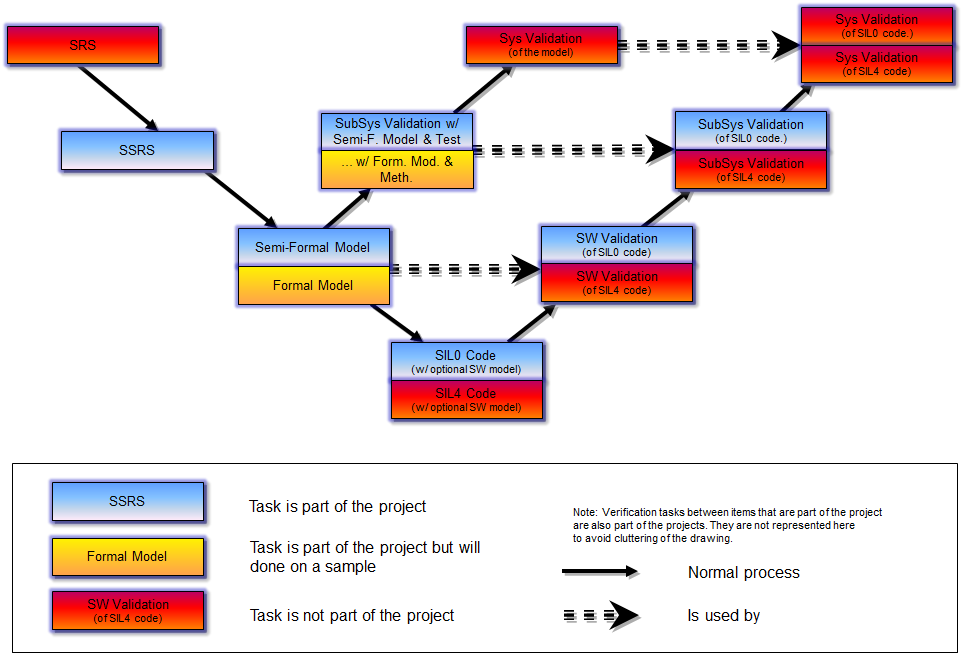
\includegraphics[scale=0.65]{Process1.png}}
  \caption{Main process}
  \label{fig:main_process}
\end{figure}

Fig. \ref{fig:safety_process} shows activities that are needed for the safety analyses. It should 
be considered in parallel of the descending branch of the V, but has been put on a separate diagram for
the sake of clarity.

High level safety properties are provided, which must be refined side-to-side with each step on the 
descending branch of the V. These properties are then used for the safety analysis of the model. The 
validation (safety analyses) boxes are yellow because the full activity will not be conducted. Only 
a subset of the safety properties will be proved.

\begin{figure}
  \centering
  \fbox{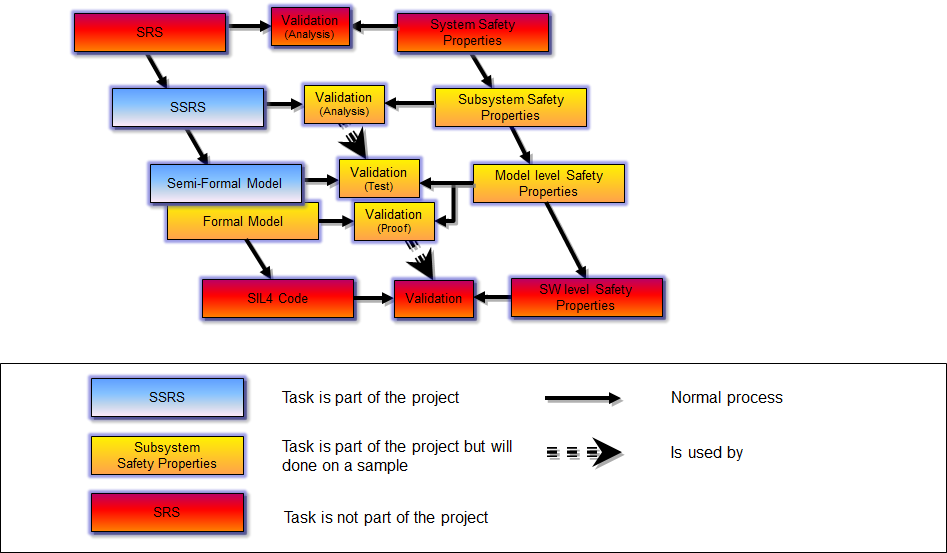
\includegraphics[scale=0.80]{Process2.png}}
  \caption{Safety analyses}
  \label{fig:safety_process}
\end{figure}

Regarding the process, WP2 shall issue (through this document) the requirements on V\&V, including
safety activities. From these requirements, WP4 shall propose the corresponding plans (Safety,
Verification and Validation). This plans will then be reviewed by WP2 to check conformance to the 
requirements. The reviewed plans will then be used as reference for the activities of the WPs.



\subsection{System specification}
\todo{To develop}
\begin{comment}This section as to define the activities links to  the system specification and model. 

This step is not explicitly defined in EN 50128 but is defined in EN 50129. However EN 50128  give the expected output from this step  for the software activities :  System  Requirements Specification, System Safety Requirements Specification, System Architecture Description, External  Interface Specifications
\end{comment}

\begin{issue}
To discuss with all partners :  Do we need a SSRS ? This is expected by EN50129.

S. Baro comments (15/02/2013) :

SSRS

We had a un-conclusive discussion on the necessity to insert a SubSystem Requirement Specification betwen the SRS (subset 26) and the formal model. The reason of this is that the model we want corresponds to a subsystem (part of the OBU), but the SRS corresponds to the whole system. The SRS also does not provide any functional architecture, and we think it is necessary to provide one. In the other hand, it adds one document between the SRS and the model. The question is thus to know if this document will remove more errors than it will add.
Proposal: To provide a SSRS which contains:
- a formal or semi-formal functional architecture of the OBU part which will be modeled, with function "boxes" and I/O "arrows";
- the requirements allocated to the functions and I/O, rewritten but still in natural language;
- the tagging Safety/Non Safety of these requirements.
This document should be seen as an important step of the modeling process, and would be under the responsibility of WP3.
 

\end{issue}

\subsection{Model definition}

\todo{To have a discussion with Sylvain Baro  on his choice of step  for the process}

\begin{comment} Some requirements to take into account :
\end{comment}

\req{The model shall be consistent with the SRS level and shall yield as
few as possible “design choices”.}
\subreq{Traceability with the SRS shall be provided. }
\subreq{Each interpretation of the SRS shall be indicated precisely.}
\subreq{Each SRS requirement not formalized in the model (\emph{e.g.} allocated to RBC)
should be traced and justified.}



\req{When the boundary of the formalized subsystem corresponds to a FIS or FFFIS, the Functional 
Architecture shall try to comply to it even when it is not mandatory.}

\req{The Functional Architecture shall split the KERNEL into independent functions.}

\req{The Functional Architecture shall identify a subset of these functions that will be modeled.}
\req{The Functional Architecture shall allow a universal method of adding function (modularity).}

\subsubsection{Software requirements}

\todo{To  detail according § 7.2 of EN 50128}

\subsubsection{Software architecture and design}

\todo{To  detail according § 7.3 of EN 50128}

\subsubsection{Software component design}

\todo{To  detail according § 7.4 of EN 50128}





\subsection{Abstract Code}

\todo{To  detail according § 7.5 of EN 50128}


\subsection{Safety activities}

\todo{this activity is not explicitly detailed in 50128 (except some task  in different activities)  but in 50126 and 50129 }

\begin{comment} from D.2.{6,7,8,9} : 
\end{comment}

\begin{justif}
Side to side with the model (which should be a dynamic model), should lay a set of  
static safety properties on the model. The higher level properties will be provided 
by the WP2 (equivalent to a preliminary hazard analysis) from the SUBSET-91 document, 

They will be refined by the safety analysis process (WP4) into properties of the same 
level than the model. The process of doing so shall be described in the Safety Plan.

This will provide Safety Properties on the model (or Dread Events). The lower level Safety Properties/
Dread Events shall address variables, state and interfaces used in the formal model.

Formal proof would then be used to prove that the OpenETCS model never enter a Dread State, 
as long as the other subsystem (RBC, communication layer\dots) fulfill their own safety properties
(axiom describing the environment).
\end{justif}

\req{A safety plan shall be provided and complied with.}
\req{The Functional Architecture shall identify the Vital and Non Vital functions.}
\begin{comment}
MPD : Identification of Vital and non vital  can be done only if the safety  analysers have provided safety properties and have allocated them to  functions.
\end{comment}
\req{The subsystem shall be compatible with the THR required in the SUBSET-091.}
\req{The safety analysis shall consider the Dread Event of the SUBSET-091, restricted to the
scope of the subsystem.}
\req{The model-level safety properties shall be written in a formal language.}

\begin{issue}
To discuss with all partners :  what is expected on this activity in the process.

S. Baro comments (15/02/2013) :

Safety

Are safety activities required in this project? The project require "certifiability" of some items (toolchain? model?) and compliance to 50128. For the toolchain, it is quite clear what it means, but for the model it is much more complicated. Is it really required for the model? If safety activities are required on the model, I think it makes no sense to refer only to 50128: it should refer to 50126 and 50129 too (excluding the hardware part which is not in the scope of the project). This pulls system safety analysis, safety properties,... but provides the initial properties required for formal proof on the model (once refined through system safety analysis).
Proposal: The "Safety" WP provides a safety case concept and safety plan according to Merlin's document and to the requirements. It is not realistic to expect that the full safety case will be provided for OpenETCS, but I think it will be useful to conduct a sample of the tasks, or all tasks but on a sample of the model. The higher level properties will be provided by subset 91, and refined by the safety analysis to properties on the model (I provided an example on how to do this in another document). Please note that even covering the whole subset 91 properties is certainly not sufficient to ensure the safety of the model.
Question: who will provide the manpower for safety activities? WP4? 

\end{issue}


\subsection{Verification and Validation}


The Verification and Validation activities have to be planned on the whole process according the requirement of EN50128 § 6.2 and 6.3.

This plan is out of the scope of the document and shall be defined in the WP4 process.

\todo{To check the existing draft on this subject}


